\section{Marcadores}
\label{sec:marcadores}

	Atualmente, é possível encontrar aplicações que utilizam padrões de símbolos bidimensionais para
	compor informações e transportar as mesmas de uma forma mais simplificada, a exemplo dos
	padrões~\textit{QRCode, PDF147} e~\textit{DataMatrix}~\cite{gao}. Alguns padrões permitem que as
	informações estejam representadas de forma redundante, pois auxiliam em sua detecção e na correção
	de possíveis erros. No âmbito industrial, seu campo de aplicação varia de acordo com a necessidade
	de cada sistema, como por exemplo transportar informações em etiquetas. Outros tipos de marcadores
	são utilizados para representar dados de localização e reconhecimento de objetos, como visto na
	Realidade Aumentada.
	
\subsection{Símbolos bidimensionais}
	\label{sec:simbolos_bidimensionais}
	
	Esse tipo de código de barras foi desenvolvido por volta de 1987. No código de barras bidimensional
	as informações são armazenadas tanto na altura quanto na largura, por essa razão possui uma maior
	capacidade de armazenamento das informações quando comparada aos símbolos unidimensionais. Os
	modelos de códigos unidimensionais armazenam as informações em apenas em uma dimensão, por
	causa dessa característica há uma limitação na quantidade de informação ser armazenada
	por eles, de acordo com cada padrão.  
	
	Para exemplificar essas características é apresentada a figura~\ref{fig:simbolos} ilustrando
	esses dois tipos de símbolos. O código apresentado na figura~\ref{fig:barcode} corresponde a um
	símbolo unidimensional, a altura desse símbolo (representado no eixo vertical) fornece
	redundância e legibilidade, possibilitando um tempo de resposta rápida, uma vez que a análise é
	feita em uma dimensão. Devido a limitação no armazenamento das informações por ele, geralmente são
	guardados valores chaves que possibilitem a busca de informações correspondentes ao código em um
	banco de dados específico. A figura~\ref{fig:datamatrix} apresenta um símbolo bidimensional
	denominado~\textit{DataMatrix}, as informações contidas neste são armazenadas em ambos os eixos
	horizontal e vertical, otimizando o espaço utilizado por ele, possibilitando a inserção de
	caracteres alfanuméricos, bem como um mecanismo responsável pela correção das informações obtidas
	através do processo de decodificação. Em contraste com esse modelo encontrado nos códigos
	unidimensionais, as informações armazenadas por esse símbolo remete a um conceito de banco de dados
	portátil e não somente o conceito de chave como apresentado no modelo unidimensional, podendo 
	armazenar uma maior quantidade de informação~\cite{gao}.
	
	\begin{figure}[htb]
		\centering
			\subfloat[\textit{BarCode} \cite{ean13}]{
				\label{fig:barcode}
				\centering 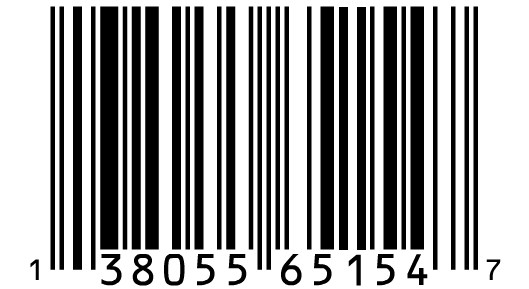
\includegraphics[scale=0.3]{figuras/cap2/codigo_barras.jpg}
			}
			\subfloat[\textit{DataMatrix} \cite{gao}]{
				\label{fig:datamatrix}
				\centering 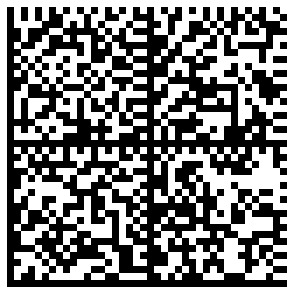
\includegraphics[scale=0.4]{figuras/cap2/datamatrix.jpg}
			}
		\caption{\textit{Exemplos de símbolos unidimensional e bidimensional.}}
		\label{fig:simbolos} 
	\end{figure}
	
	Os códigos bidimensionais podem ser divididos em duas categorias. A primeira denominada
	~\textit{stacked code} e a segunda chamada de~\textit{matrix code}. A diferença entre essas
	categorias está na sua composição. Enquanto que a~\textit{stacked code} trabalha com simbologias
	compostas por uma série de código de barras unidimensionais empilhadas uma em cima das outras,
	a~\textit{matrix code} codifica os dados com base nas posições dos pontos negros definidos dentro
	de uma matriz. Isso faz com que cada elemento da matriz possua a mesma dimensão, desta forma a
	decodificação é calculada em relação a posição do elemento preenchido na matriz. A
	tabela~\ref{tab:exemplo} apresenta alguns tipos de códigos bidimensionais e a categoria
	correspondente a cada código listado.
	
	
	\begin{table} % aqui começa o ambiente tabela
		\centering
		\caption{Códigos bidimensionais e suas categorias.}
		\begin{tabular}{lcc} 
			\hline % este comando coloca uma linha na tabela
			\textbf{Código bidimensional} & \textbf{Categoria} \\ 
			%\textit{\textbf{Stacked code}} & \textit{\textbf{Matrix code}}	\\
			\hline
			\hline
			\textit{Code 49} & \textit{Stacked} \\
			\textit{Data Matrix} & \textit{\textit{Matrix}} \\
			\textit{Portable Data File 417 (PDF417)} & \textit{Stacked}  \\
			\textit{QRCode} & \textit{\textit{Matrix}}\\
			\hline
		\end{tabular}
		\label{tab:exemplo}
	\end{table}
	
	A figura \ref{fig:qrCode} exemplifica um código de barras bidimensional da 
	categoria~\textit{matrix code}. Esse tipo de código é denominado de \textit{QRCode (Quick Response Code)}. 
	O \textit{QRCode} foi desenvolvido no Japão, no ano de 1994 com o objetivo de ser um código que possibilitasse um
	bom armazenamento de informações, compacto e que oferecesse uma leitura rápida e de fácil acesso.
	Este código pode codificar até 7089 caracteres numéricos (somente números), 4296 caracteres alfanuméricos 
	(letras e caracteres ASCII) ou 2953 \textit{bytes} de dados binários (\textit{bytes} hexadecimal)~\cite{kato}. Possui um 
	formato quadrático com dimensões variando
	de 21 x 21 até 177 x 177 células (conforme a versão do~\textit{QRCode}), onde cada célula codifica
	um \textit{bit}. É oferecido quatro níveis de detecção e correção de erros, possibilitando a
	recuperação de informações de regiões danificadas do código. A tabela~\ref{tab:nivelFalha}
	exemplifica esses níveis e apresenta a porcentagem de recuperação das informações oferecida por
	cada nível.
	
	
	\begin{table}
		\centering
		\caption{Níveis de correção de erros suportado pelo QRCode~\cite{kato}.}
		\begin{tabular}{lcc} 
			\hline
			 \textbf{Nível} & \textbf{Porcentagem de informação recuperada} \\
			\hline
			\hline
			\textit{Low} & 7\% \\
			\textit{Medium} & 15\% \\
			\textit{Quality} & 25\% \\
			\textit{High} & 30\% \\
			\hline
		\end{tabular}
		\label{tab:nivelFalha}
	\end{table}
	
	
	O \textit{QRCode} possui características estruturais com o objetivo de facilitar sua identificação
	e obtenção das informações necessárias para a sua correta decodificação. Tais características
	estão ilustradas na figura~\ref{fig:qrCode}.
				
	\begin{figure}[htb]
		\centering 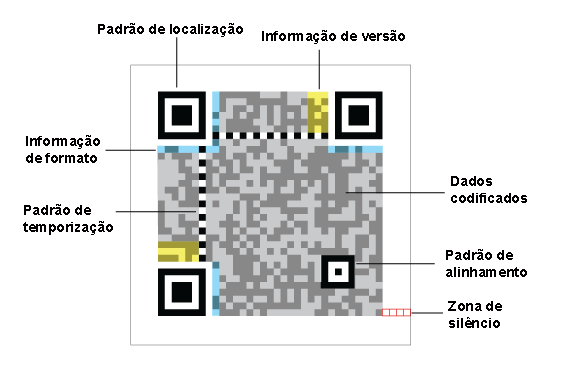
\includegraphics[scale=0.6]{figuras/cap2/qranatomy.png}
		\caption{\textit{Ilustração das propriedades estruturais do QRCode. Adaptado de~\cite{qrcodespec}.}}
		\label{fig:qrCode} 
	\end{figure} 
	
	\begin{itemize}
	  \item \textit{Padrão de localização}
			  
	  	Esse padrão baseia-se nas posições dos três vértices localizadas nos cantos do símbolo. A
	  	partir desses três pontos é possível estimar o quarto canto da imagem, por consequência a
	  	posição, tamanho e o centro dos símbolos podem ser detectados, sendo assim utilizado para
	  	referência posicional do símbolo. Desta forma, o reconhecimento pode ser feito em todas as
	  	direções.
				  
		\item \textit{Padrão de temporização}
				  
		Padrão responsável pela identificação e correção das coordenadas centrais de cada célula. Este
		padrão é utilizado quando o símbolo está distorcido, possibilitando a identificação do espaçamento
		entre as células.
					
		\item \textit{Padrão de alinhamento}
					
		Por fim, a correção de distorção, especialmente a não linear, é feita através desse padrão. 
		Essa visa corrigir a distorção do símbolo quando este estiver em uma superfície curva ou 
		com o leitor inclinado.	Por fim, esta célula facilita a obtenção da coordenada central do padrão 
		de alinhamento.
		
		\item \textit{Dados codificados}
		
		É a região responsável pelo armazenamento dos dados codificados.
		
		\item \textit{Informação de formato}
		
		Contém a taxa de correção de erro e o padrão de máscara utilizado.
		
		\item \textit{Zona de silêncio}
		
		É a margem ao redor do \textit{QRCode} necessário para que o código seja lido corretamente. Possui
		a medida correspondente a quatro células de largura.
		
		\item \textit{Informação de versão}
		
		Responsável pela identificação da versão utilizada pelo \textit{QRCode}, podendo variar a partir
		da versão 1 (correspondente a 21 x 21 células) até a versão 40 (correspondente a 177 x 177
		células). As versões possuem a mesma estrutura, porém a capacidade de armazenamento varia de uma
		versão para outra.
									
	\end{itemize}
	
	A tabela \ref{tab:tabelaCodigos} mostra um comparativo entre diferentes tipos de códigos tanto
	unidimensionais (\textit{barcode}) quanto bidimensionais (\textit{QRCode} e \textit{Data Matrix}).
	As quantidade de referência internas apresentadas na tabela dizem respeito a pontos contidos
	internamente dentro do código cujo propósito seja o auxílio para obtenção do correto
 	posicionamento do mesmo. Também é mostrada a diferença na quantidade de informação armazenada por
	esses códigos.
	
	
	\begin{table} % aqui começa o ambiente tabela
		\centering
		\caption{Comparação de vários códigos \cite{marlon}.}
		\begin{tabular}{lccc} 
			\hline % este comando coloca uma linha na tabela
			 & \textbf{\textit{Barcode}} & \textbf{QRCode} & \textbf{\textit{DataMatrix}} \\
			\hline
			\hline
			Capacidade de armazenamento & 1\textit{byte}/4cm	 & 2953 \textit{bytes} & 2335 \textit{bytes} \\
			Velocidade de leitura & Rápido & Rápido & Lenta\\
			Especificação aberta & Sim & Sim & Sim\\
			Referências internas & 0 & 3 & 2 \\ 
			Recuperação dos dados & Não & Até 30 \%  & Até 30 \% \\
			Formato & Linear & Quadrado & Retangular\\
			\hline
		\end{tabular}
		 % igual ao ambiente figura
		\label{tab:tabelaCodigos}
	\end{table}
	
\subsection{Marcadores para Realidade Aumentada}
\label{sec:marcadoresRA}
		
		Cada aplicação voltada para a criação e/ou detecção de marcadores pode possuir seus próprios
		padrões de marcadores e algoritmos para seu reconhecimento. A área de definição de marcadores
		utilizados ainda está em aberto, com espaço para melhorias de acordo com cada aplicação~\cite{fpga}. Dentro
		desse universo pode-se citar as aplicações ARToolkit~\cite{artoolkit}, ARTag~\cite{artag} e
		ARToolkitPlus~\cite{kler}.
		
		De uma forma geral, para os objetos sejam reconhecidos como potenciais marcadores por
		essas aplicações, estes necessitam de um formato padrão constituído por uma ``moldura''
		confeccionada com bordas quadradas, de preferência na cor preta, pois algumas aplicações convertem
		as cores da imagem em uma escala de cinza. A construção e decodificação do conteúdo interior do
		marcador pode variar de acordo com cada aplicação, possibilitando uma flexibilização na construção
		do mesmo. Na abordagem da aplicação ARToolkit, o centro desses marcadores pode ser constituído por
		uma figura. Já no ARToolkitPlus, o interior dos marcadores é preenchido por quadrados de cor
		preta, podendo formar figuras geométricas diversas. Exemplos de marcadores utilizados por essas
		aplicações são apresentados na figura~\ref{fig:marcadoresAR}. 
		
		\begin{figure}[htb]
			\centering
				\subfloat[ARToolKit \cite{artoolkit}]{
					\label{fig:artoolkit}
					\centering 
\includegraphics[scale=1]{figuras/cap2/arToolkitMarker.png}
				}
				\subfloat[ARTag \cite{artag}]{
					\label{fig:artag}
					\centering 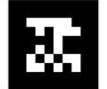
\includegraphics[scale=1]{figuras/cap2/arTagMarker.png}
				}
				\subfloat[ARToolkitPlus \cite{kler}]{
					\label{fig:artoolkitplus}
					\centering 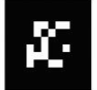
\includegraphics[scale=1]{figuras/cap2/arToolkitPlusMarker.png}
				}
			\caption{\textit{Exemplo de alguns marcadores utilizados na realidade aumentada.}}
			\label{fig:marcadoresAR} 
		\end{figure}
		
	Fazendo uma comparação entre esses marcadores e o \textit{QRCode} é possível observar que, da mesma
	forma como acontece com o código unidimensional apresentado na tabela~\ref{tab:tabelaCodigos},
	estes não possibilitam a recuperação de informações danificadas, mas possibilitam a identificação do erro. 
	Desta forma o não reconhecimento de parte do marcador pode comprometer todo o processo de reconhecimento. 
	Diferentemente do \textit{QRCode}, esses marcadores possuem uma capacidade bastante limitada para 
	armazenamento de informações. Por causa dessa limitação a maioria dos marcadores guardam somente um código
	identificador. Entretanto, são menos sensíveis a distorções de ângulo devido sua simplicidade. 
	
